% Options for packages loaded elsewhere
\PassOptionsToPackage{unicode}{hyperref}
\PassOptionsToPackage{hyphens}{url}
%
\documentclass[
]{article}
\usepackage{lmodern}
\usepackage{amssymb,amsmath}
\usepackage{ifxetex,ifluatex}
\ifnum 0\ifxetex 1\fi\ifluatex 1\fi=0 % if pdftex
  \usepackage[T1]{fontenc}
  \usepackage[utf8]{inputenc}
  \usepackage{textcomp} % provide euro and other symbols
\else % if luatex or xetex
  \usepackage{unicode-math}
  \defaultfontfeatures{Scale=MatchLowercase}
  \defaultfontfeatures[\rmfamily]{Ligatures=TeX,Scale=1}
\fi
% Use upquote if available, for straight quotes in verbatim environments
\IfFileExists{upquote.sty}{\usepackage{upquote}}{}
\IfFileExists{microtype.sty}{% use microtype if available
  \usepackage[]{microtype}
  \UseMicrotypeSet[protrusion]{basicmath} % disable protrusion for tt fonts
}{}
\makeatletter
\@ifundefined{KOMAClassName}{% if non-KOMA class
  \IfFileExists{parskip.sty}{%
    \usepackage{parskip}
  }{% else
    \setlength{\parindent}{0pt}
    \setlength{\parskip}{6pt plus 2pt minus 1pt}}
}{% if KOMA class
  \KOMAoptions{parskip=half}}
\makeatother
\usepackage{xcolor}
\IfFileExists{xurl.sty}{\usepackage{xurl}}{} % add URL line breaks if available
\IfFileExists{bookmark.sty}{\usepackage{bookmark}}{\usepackage{hyperref}}
\hypersetup{
  pdftitle={MATH 1051H-A: Lecture \#07},
  pdfauthor={Wesley Burr},
  hidelinks,
  pdfcreator={LaTeX via pandoc}}
\urlstyle{same} % disable monospaced font for URLs
\usepackage[margin=1in]{geometry}
\usepackage{color}
\usepackage{fancyvrb}
\newcommand{\VerbBar}{|}
\newcommand{\VERB}{\Verb[commandchars=\\\{\}]}
\DefineVerbatimEnvironment{Highlighting}{Verbatim}{commandchars=\\\{\}}
% Add ',fontsize=\small' for more characters per line
\usepackage{framed}
\definecolor{shadecolor}{RGB}{248,248,248}
\newenvironment{Shaded}{\begin{snugshade}}{\end{snugshade}}
\newcommand{\AlertTok}[1]{\textcolor[rgb]{0.94,0.16,0.16}{#1}}
\newcommand{\AnnotationTok}[1]{\textcolor[rgb]{0.56,0.35,0.01}{\textbf{\textit{#1}}}}
\newcommand{\AttributeTok}[1]{\textcolor[rgb]{0.77,0.63,0.00}{#1}}
\newcommand{\BaseNTok}[1]{\textcolor[rgb]{0.00,0.00,0.81}{#1}}
\newcommand{\BuiltInTok}[1]{#1}
\newcommand{\CharTok}[1]{\textcolor[rgb]{0.31,0.60,0.02}{#1}}
\newcommand{\CommentTok}[1]{\textcolor[rgb]{0.56,0.35,0.01}{\textit{#1}}}
\newcommand{\CommentVarTok}[1]{\textcolor[rgb]{0.56,0.35,0.01}{\textbf{\textit{#1}}}}
\newcommand{\ConstantTok}[1]{\textcolor[rgb]{0.00,0.00,0.00}{#1}}
\newcommand{\ControlFlowTok}[1]{\textcolor[rgb]{0.13,0.29,0.53}{\textbf{#1}}}
\newcommand{\DataTypeTok}[1]{\textcolor[rgb]{0.13,0.29,0.53}{#1}}
\newcommand{\DecValTok}[1]{\textcolor[rgb]{0.00,0.00,0.81}{#1}}
\newcommand{\DocumentationTok}[1]{\textcolor[rgb]{0.56,0.35,0.01}{\textbf{\textit{#1}}}}
\newcommand{\ErrorTok}[1]{\textcolor[rgb]{0.64,0.00,0.00}{\textbf{#1}}}
\newcommand{\ExtensionTok}[1]{#1}
\newcommand{\FloatTok}[1]{\textcolor[rgb]{0.00,0.00,0.81}{#1}}
\newcommand{\FunctionTok}[1]{\textcolor[rgb]{0.00,0.00,0.00}{#1}}
\newcommand{\ImportTok}[1]{#1}
\newcommand{\InformationTok}[1]{\textcolor[rgb]{0.56,0.35,0.01}{\textbf{\textit{#1}}}}
\newcommand{\KeywordTok}[1]{\textcolor[rgb]{0.13,0.29,0.53}{\textbf{#1}}}
\newcommand{\NormalTok}[1]{#1}
\newcommand{\OperatorTok}[1]{\textcolor[rgb]{0.81,0.36,0.00}{\textbf{#1}}}
\newcommand{\OtherTok}[1]{\textcolor[rgb]{0.56,0.35,0.01}{#1}}
\newcommand{\PreprocessorTok}[1]{\textcolor[rgb]{0.56,0.35,0.01}{\textit{#1}}}
\newcommand{\RegionMarkerTok}[1]{#1}
\newcommand{\SpecialCharTok}[1]{\textcolor[rgb]{0.00,0.00,0.00}{#1}}
\newcommand{\SpecialStringTok}[1]{\textcolor[rgb]{0.31,0.60,0.02}{#1}}
\newcommand{\StringTok}[1]{\textcolor[rgb]{0.31,0.60,0.02}{#1}}
\newcommand{\VariableTok}[1]{\textcolor[rgb]{0.00,0.00,0.00}{#1}}
\newcommand{\VerbatimStringTok}[1]{\textcolor[rgb]{0.31,0.60,0.02}{#1}}
\newcommand{\WarningTok}[1]{\textcolor[rgb]{0.56,0.35,0.01}{\textbf{\textit{#1}}}}
\usepackage{longtable,booktabs}
% Correct order of tables after \paragraph or \subparagraph
\usepackage{etoolbox}
\makeatletter
\patchcmd\longtable{\par}{\if@noskipsec\mbox{}\fi\par}{}{}
\makeatother
% Allow footnotes in longtable head/foot
\IfFileExists{footnotehyper.sty}{\usepackage{footnotehyper}}{\usepackage{footnote}}
\makesavenoteenv{longtable}
\usepackage{graphicx,grffile}
\makeatletter
\def\maxwidth{\ifdim\Gin@nat@width>\linewidth\linewidth\else\Gin@nat@width\fi}
\def\maxheight{\ifdim\Gin@nat@height>\textheight\textheight\else\Gin@nat@height\fi}
\makeatother
% Scale images if necessary, so that they will not overflow the page
% margins by default, and it is still possible to overwrite the defaults
% using explicit options in \includegraphics[width, height, ...]{}
\setkeys{Gin}{width=\maxwidth,height=\maxheight,keepaspectratio}
% Set default figure placement to htbp
\makeatletter
\def\fps@figure{htbp}
\makeatother
\setlength{\emergencystretch}{3em} % prevent overfull lines
\providecommand{\tightlist}{%
  \setlength{\itemsep}{0pt}\setlength{\parskip}{0pt}}
\setcounter{secnumdepth}{-\maxdimen} % remove section numbering

\title{MATH 1051H-A: Lecture \#07}
\author{Wesley Burr}
\date{10/02/2020}

\begin{document}
\maketitle

\hypertarget{random-variables}{%
\section{Random variables}\label{random-variables}}

\hypertarget{random-variables-1}{%
\subsection{Random variables}\label{random-variables-1}}

\begin{itemize}
\tightlist
\item
  A \textbf{random variable} is a numeric quantity whose value depends
  on the outcome of a random event

  \begin{itemize}
  \tightlist
  \item
    We use a capital letter, like \(X\), to denote a random variable
  \item
    The values of a random variable are denoted with a lowercase letter,
    in this case \(x\)
  \item
    We write this as \(P(X = x)\)
  \end{itemize}
\end{itemize}

\hypertarget{random-variables-2}{%
\subsection{Random variables}\label{random-variables-2}}

\begin{itemize}
\tightlist
\item
  A \textbf{random variable} is a numeric quantity whose value depends
  on the outcome of a random event

  \begin{itemize}
  \tightlist
  \item
    We use a capital letter, like \(X\), to denote a random variable
  \item
    The values of a random variable are denoted with a lowercase letter,
    in this case \(x\)
  \item
    We write this as \(P(X = x)\)
  \end{itemize}
\item
  There are two types of random variables:

  \begin{itemize}
  \tightlist
  \item
    \textbf{Discrete random variables} often take only integer values

    \begin{itemize}
    \tightlist
    \item
      \textbf{Example}: Number of credit hours, Difference in number of
      credit hours this term vs last
    \end{itemize}
  \item
    \textbf{Continuous random variables} take real (decimal) values

    \begin{itemize}
    \tightlist
    \item
      \textbf{Example}: Cost of books this term, Difference in cost of
      books this term vs last
    \end{itemize}
  \end{itemize}
\end{itemize}

\hypertarget{expectation}{%
\subsection{Expectation}\label{expectation}}

\begin{itemize}
\tightlist
\item
  We are often interested in the average outcome of a random variable.
\item
  We call this the \textbf{expected value}, or \textbf{mean}, and it is
  a weighted average of the possible outcomes \[
  \mu = E(X) = \sum_{i = 1}^k x_i ~ P(X = x_i)
  \]
\end{itemize}

\hypertarget{expected-value-of-a-discrete-random-variable}{%
\subsection{Expected value of a discrete random
variable}\label{expected-value-of-a-discrete-random-variable}}

In a game of cards you win \$1 if you draw a heart, \$5 if you draw an
ace (including the ace of hearts), \$10 if you draw the king of spades
and nothing for any other card you draw. Write the probability model for
your winnings, and calculate your expected winning.

\begin{longtable}[]{@{}lrcr@{}}
\toprule
Event & \(X\) & \(P(X)\) & \(X ~ P(X)\)\tabularnewline
\midrule
\endhead
Heart (not ace) & \(1\) & 12/52 & 12/52\tabularnewline
Ace & \(5\) & 4/52 & 20/52\tabularnewline
King of spades & \(10\) & 1/52 & 10/52\tabularnewline
All else & \(0\) & 35/52 & 0\tabularnewline
\bottomrule
\end{longtable}

\hypertarget{expected-value-of-a-discrete-random-variable-1}{%
\subsection{Expected value of a discrete random
variable}\label{expected-value-of-a-discrete-random-variable-1}}

\begin{longtable}[]{@{}lrcr@{}}
\toprule
Event & \(X\) & \(P(X)\) & \(X ~ P(X)\)\tabularnewline
\midrule
\endhead
Heart (not ace) & \(1\) & 12/52 & 12/52\tabularnewline
Ace & \(5\) & 4/52 & 20/52\tabularnewline
King of spades & \(10\) & 1/52 & 10/52\tabularnewline
All else & \(0\) & 35/52 & 0\tabularnewline
Total & & & \(E[X] = 42/52 \approx 0.81\)\tabularnewline
\bottomrule
\end{longtable}

\hypertarget{expected-value-of-a-discrete-random-variable-cont.}{%
\subsection{Expected value of a discrete random variable
(cont.)}\label{expected-value-of-a-discrete-random-variable-cont.}}

Below is a visual representation of the probability distribution of
winnings from this game:

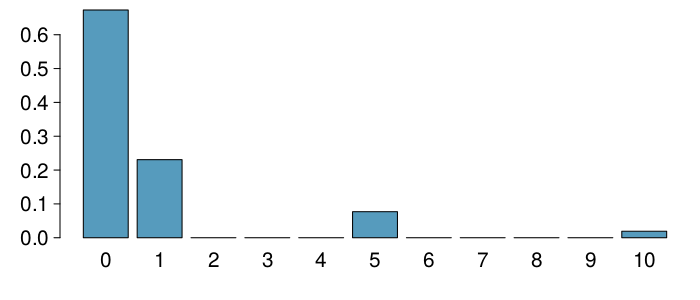
\includegraphics[width=700px]{fig/card_game}

\hypertarget{variability-in-random-variables}{%
\subsection{Variability in random
variables}\label{variability-in-random-variables}}

We are also often interested in the variability in the values of a
random variable.

\[
\sigma^2 = Var(X) = \sum_{i = 1}^k \left(x_i - E(X)\right)^2 P(X = x_i)\\
\;\\
\sigma = SD(X) = \sqrt{Var(X)}
\]

\hypertarget{variability-of-a-discrete-random-variable}{%
\subsection{Variability of a discrete random
variable}\label{variability-of-a-discrete-random-variable}}

\textbf{For the previous card game example, how much would you expect
the winnings to vary from game to game?}

\begin{longtable}[]{@{}lllll@{}}
\toprule
\(X\) & \(P(X)\) & \(X~P(X)\) & \((X-E[X])^2\) &
\(P(X)\cdot (X-E[X])^2\)\tabularnewline
\midrule
\endhead
1 & 12/52 & 1 x 12/52 = 12/52 & \$(1-0.81)\^{}2 = 0.0361 & 12/52 x
0.0361 = 0.0083\tabularnewline
5 & 4/52 & 5 x 4/52 = 20/52 & \$(5-0.81)\^{}2 = 17.5561 & 4/52 x 17.5561
= 1.3505\tabularnewline
10 & 1/52 & 10 x 1/52 = 10/52 & \$(10-0.81)\^{}2 = 84.4561 & 1/52 x
84.0889 = 1.6242\tabularnewline
0 & 35/52 & 0 x 35/52 = 0 & \$(0-0.81)\^{}2 = 0.6561 & 35/52 x 0.6561 =
0.4416\tabularnewline
& & \(E[X] = 0.81\) & &\tabularnewline
\bottomrule
\end{longtable}

\hypertarget{variability-of-a-discrete-random-variable-1}{%
\subsection{Variability of a discrete random
variable}\label{variability-of-a-discrete-random-variable-1}}

\textbf{For the previous card game example, how much would you expect
the winnings to vary from game to game?}

\begin{longtable}[]{@{}lllll@{}}
\toprule
\(X\) & \(P(X)\) & \(X~P(X)\) & \((X-E[X])^2\) &
\(P(X)\cdot (X-E[X])^2\)\tabularnewline
\midrule
\endhead
1 & 12/52 & 1 x 12/52 = 12/52 & \$(1-0.81)\^{}2 = 0.0361 & 12/52 x
0.0361 = 0.0083\tabularnewline
5 & 4/52 & 5 x 4/52 = 20/52 & \$(5-0.81)\^{}2 = 17.5561 & 4/52 x 17.5561
= 1.3505\tabularnewline
10 & 1/52 & 10 x 1/52 = 10/52 & \$(10-0.81)\^{}2 = 84.4561 & 1/52 x
84.0889 = 1.6242\tabularnewline
0 & 35/52 & 0 x 35/52 = 0 & \$(0-0.81)\^{}2 = 0.6561 & 35/52 x 0.6561 =
0.4416\tabularnewline
& & \(E[X] = 0.81\) & & \(V[X] = 3.4246\)\tabularnewline
& & & & \(SD(X) = \sqrt{3.4246} = 1.85\)\tabularnewline
\bottomrule
\end{longtable}

\hypertarget{variability-the-r-way}{%
\subsection{Variability: the R way}\label{variability-the-r-way}}

We could also do all of this in R, and it's easier: no tracking
decimals, no computations!

\begin{Shaded}
\begin{Highlighting}[]
\NormalTok{x <-}\StringTok{ }\KeywordTok{c}\NormalTok{(}\DecValTok{1}\NormalTok{, }\DecValTok{5}\NormalTok{, }\DecValTok{10}\NormalTok{, }\DecValTok{0}\NormalTok{)}
\NormalTok{pX <-}\StringTok{ }\KeywordTok{c}\NormalTok{(}\DecValTok{12}\OperatorTok{/}\DecValTok{52}\NormalTok{, }\DecValTok{4}\OperatorTok{/}\DecValTok{52}\NormalTok{, }\DecValTok{1}\OperatorTok{/}\DecValTok{52}\NormalTok{, }\DecValTok{35}\OperatorTok{/}\DecValTok{52}\NormalTok{)}
\NormalTok{var <-}\StringTok{ }\NormalTok{pX }\OperatorTok{*}\StringTok{ }\NormalTok{(x }\OperatorTok{-}\StringTok{ }\KeywordTok{sum}\NormalTok{(x }\OperatorTok{*}\StringTok{ }\NormalTok{pX))}\OperatorTok{^}\DecValTok{2}
\NormalTok{var}
\end{Highlighting}
\end{Shaded}

\begin{verbatim}
## [1] 0.008534365 1.351957214 1.624971552 0.439093081
\end{verbatim}

\begin{Shaded}
\begin{Highlighting}[]
\KeywordTok{sum}\NormalTok{(var)}
\end{Highlighting}
\end{Shaded}

\begin{verbatim}
## [1] 3.424556
\end{verbatim}

\hypertarget{linear-combinations-of-random-variables}{%
\subsection{Linear combinations of random
variables}\label{linear-combinations-of-random-variables}}

\begin{itemize}
\tightlist
\item
  A \textbf{linear combination} of random variables \(X\) and \(Y\) is
  given by \[
  aX + bY 
  \] where \(a\) and \(b\) are some fixed numbers.
\end{itemize}

\hypertarget{linear-combinations-of-random-variables-1}{%
\subsection{Linear combinations of random
variables}\label{linear-combinations-of-random-variables-1}}

\begin{itemize}
\tightlist
\item
  A \textbf{linear combination} of random variables \(X\) and \(Y\) is
  given by \[
  aX + bY 
  \] where \(a\) and \(b\) are some fixed numbers.
\item
  The average value of a linear combination of random variables is given
  by \[
  E(aX + bY) = a \times E(X) + b \times E(Y)
  \]
\end{itemize}

\hypertarget{calculating-the-expectation-of-a-linear-combination}{%
\subsection{Calculating the expectation of a linear
combination}\label{calculating-the-expectation-of-a-linear-combination}}

On average you take 10 minutes for each statistics homework problem and
15 minutes for each chemistry homework problem. This week you have 5
statistics and 4 chemistry homework problems assigned. What is the total
time you expect to spend on statistics and physics homework for the
week?

\hypertarget{calculating-the-expectation-of-a-linear-combination-1}{%
\subsection{Calculating the expectation of a linear
combination}\label{calculating-the-expectation-of-a-linear-combination-1}}

On average you take 10 minutes for each statistics homework problem and
15 minutes for each chemistry homework problem. This week you have 5
statistics and 4 chemistry homework problems assigned. What is the total
time you expect to spend on statistics and physics homework for the
week?

\[
\begin{split}
E(S + S + S + S + S + C + C + C + C) &= 5 \times E(S) + 4 \times E(C) \\
&= 5 \times 10 + 4 \times 15 \\
&= 50 + 60 \\
&= 110~\text{min }
\end{split}
\]

\hypertarget{variability-in-linear-combinations-of-random-variables}{%
\subsection{Variability in linear combinations of random
variables}\label{variability-in-linear-combinations-of-random-variables}}

\begin{itemize}
\tightlist
\item
  The variability of a linear combination of two independent random
  variables is calculated as \[
  V(aX + bY) = a^2 \times V(X) + b^2 \times V(Y)
  \]
\item
  The standard deviation of the linear combination is the square root of
  the variance.
\end{itemize}

\textbf{If the random variables are not independent, the variance
calculation gets a little more complicated and is beyond the scope of
this course.}

\hypertarget{calculating-the-variance-of-a-linear-combination}{%
\subsection{Calculating the variance of a linear
combination}\label{calculating-the-variance-of-a-linear-combination}}

The standard deviation of the time you take for each statistics homework
problem is 1.5 minutes, and it is 2 minutes for each chemistry problem.
What is the standard deviation of the time you expect to spend on
statistics and physics homework for the week if you have 5 statistics
and 4 chemistry homework problems assigned? Suppose that the time it
takes to complete each problem is independent of another.

\hypertarget{calculating-the-variance-of-a-linear-combination-1}{%
\subsection{Calculating the variance of a linear
combination}\label{calculating-the-variance-of-a-linear-combination-1}}

The standard deviation of the time you take for each statistics homework
problem is 1.5 minutes, and it is 2 minutes for each chemistry problem.
What is the standard deviation of the time you expect to spend on
statistics and physics homework for the week if you have 5 statistics
and 4 chemistry homework problems assigned? Suppose that the time it
takes to complete each problem is independent of another.

\[
\begin{split}
V(S+S+S+S+S+C+C+C) &= V(S) + V(S) + V(S) + V(S) + \\ &\phantom{==}V(S) + V(C) + V(C) + V(C) + V(C) \\
&= 5 \times V(S) + 4 \times V(C) \\
&= 5 \times 1.5^2 + 4 \times 2^2 \\
&= 27.25
\end{split}
\]

\hypertarget{calculating-variance-the-r-way}{%
\subsection{Calculating Variance: the R
way}\label{calculating-variance-the-r-way}}

\begin{Shaded}
\begin{Highlighting}[]
\DecValTok{5} \OperatorTok{*}\StringTok{ }\FloatTok{1.5}\OperatorTok{^}\DecValTok{2} \OperatorTok{+}\StringTok{ }\DecValTok{4} \OperatorTok{*}\StringTok{ }\DecValTok{2}\OperatorTok{^}\DecValTok{2}
\end{Highlighting}
\end{Shaded}

\begin{verbatim}
## [1] 27.25
\end{verbatim}

\hypertarget{practice}{%
\subsection{Practice}\label{practice}}

A casino game costs \$5 to play. If the first card you draw is red, then
you get to draw a second card (without replacement). If the second card
is the ace of clubs, you win \$500. If not, you don't win anything,
i.e.~lose your \$5. What is your expected profits/losses from playing
this game? \textbf{{Remember: profit/loss = winnings - cost.}}

\begin{itemize}
\tightlist
\item
  A profit of 5 cents
\item
  A loss of 10 cents
\item
  A loss of 25 cents
\item
  A loss of 30 cents
\end{itemize}

\hypertarget{practice-1}{%
\subsection{Practice}\label{practice-1}}

A casino game costs \$5 to play. If the first card you draw is red, then
you get to draw a second card (without replacement). If the second card
is the ace of clubs, you win \$500. If not, you don't win anything,
i.e.~lose your \$5. What is your expected profits/losses from playing
this game? \textbf{{Remember: profit/loss = winnings - cost.}}

\[
\text{A profit of 5 cents}\qquad \text{A loss of 25 cents}\\
\text{A loss of 10 cents} \qquad \text{A loss of 30 cents}
\]

\begin{longtable}[]{@{}lllll@{}}
\toprule
Event & Win & Profit:\(~X\) & \(P(X)\) & \(X\cdot P(X)\)\tabularnewline
\midrule
\endhead
\textbf{Red}, A\{\(\clubsuit\)\} & 500 & \(500 - 5 = 495\) &
\(\frac{26}{52} \cdot\frac{1}{51} = 0.0098\) &
\(495 \times 0.0098 = 4.851\)\tabularnewline
Other & 0 & \(0 - 5 = -5\) & \(1 - 0.0098 = 0.9902\) &
\(-5 \times 0.9902 = -4.951\)\tabularnewline
& & & & \(E(X) = -0.1\)\tabularnewline
\bottomrule
\end{longtable}

\hypertarget{fair-game}{%
\subsection{Fair game}\label{fair-game}}

A \textbf{fair} game is defined as a game that costs as much as its
expected payout, i.e.~expected profit is 0.

\hypertarget{fair-game-1}{%
\subsection{Fair game}\label{fair-game-1}}

A \textbf{fair} game is defined as a game that costs as much as its
expected payout, i.e.~expected profit is 0.

\textbf{Do you think casino games in Vegas cost more or less than their
expected payouts?}

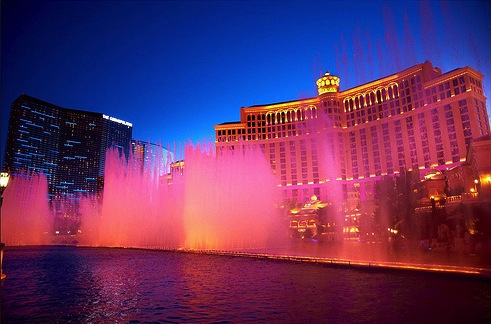
\includegraphics[width=400px]{fig/bellagio}

If those games cost less than their expected payouts, it would mean that
the casinos would be losing money on average, and hence they wouldn't be
able to pay for all this:

\hypertarget{simplifying-random-variables}{%
\subsection{Simplifying random
variables}\label{simplifying-random-variables}}

Random variables do not work like normal algebraic variables: \[
X + X \ne 2X
\]

\hypertarget{simplifying-random-variables-1}{%
\subsection{Simplifying random
variables}\label{simplifying-random-variables-1}}

Random variables do not work like normal algebraic variables: \[
X + X \ne 2X
\]

\[
\begin{align*}
E(X + X) &= E(X) + E(X) \\
&= 2 E(X) \\
&~  \\
E(2X) &= 2 E(X) \\
&~ 
\end{align*}
\]

\hypertarget{simplifying-random-variables-cont.}{%
\subsection{Simplifying random variables
(cont.)}\label{simplifying-random-variables-cont.}}

\[
\begin{align*}
Var(X + X) &= Var(X) + Var(X)~{\scriptsize \text{(assuming independence)}} \\
&= 2~Var(X) \\
&~  \\
Var(2X) &= 2^2~Var(X) \\
&= 4~Var(X)
\end{align*}
\]

\textbf{So}: \[
E(X + X)  = E(2X), \text{ but }  Var(X + X) \ne Var(2X)
\]

\hypertarget{adding-or-multiplying}{%
\subsection{Adding or multiplying?}\label{adding-or-multiplying}}

A company has 5 Lincoln Town Cars in its fleet. Historical data show
that annual maintenance cost for each car is on average \$2,154 with a
standard deviation of \$132. What is the mean and the standard deviation
of the total annual maintenance cost for this fleet?

Note that we have 5 cars each with the given annual maintenance cost
\((X_1 + X_2 + X_3 + X_4 + X_5)\), not one car that had 5 times the
given annual maintenance cost \((5X)\).

\hypertarget{adding-or-multiplying-1}{%
\subsection{Adding or multiplying?}\label{adding-or-multiplying-1}}

\[
\begin{split}
E(X_1 + X_2 + X_3 + X_4 + X_5) &=& E(X_1) + E(X_2) + \cdots + E(X_5) \\
&=& 5 \times E(X) = 5 \times 2,154 = \$ 10,770 \\
Var(X_1 + X_2 + X_3 + X_4 + X_5) &=& Var(X_1) + Var(X_2) + \cdots + Var(X_5) \\
&=& 5 \times V(X) = 5 \times 132^2 = \$ 87,120 \\
SD(X_1 + X_2 + X_3 + X_4 + X_5) &=& \sqrt{87,120} =  295.16
\end{split}
\]

\end{document}
